\begin{pastexam}[label={px:nchu-114-dsa-24}]{中興資工所甲組 114 學年度 計算題第 4 題}
（計算）

(5\%) Using Kruskal's algorithm, calculate the \textbf{total cost} of the minimum spanning tree (MST) for the graph shown.

\begin{center}
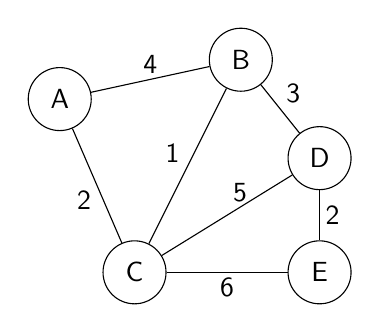
\begin{tikzpicture}[v/.style={circle,draw,minimum size=8mm,inner sep=0pt,font=\sffamily},w/.style={font=\sffamily,inner sep=2pt}]
\node[v] (A) at (0,0) {A};
\node[v] (B) at (2.3,0.5) {B};
\node[v] (D) at (3.3,-0.75) {D};
\node[v] (C) at (0.95,-2.2) {C};
\node[v] (E) at (3.3,-2.2) {E};
\draw (A) -- node[w,above] {4} (B);
\draw (B) -- node[w,above right] {3} (D);
\draw (A) -- node[w,below left] {2} (C);
\draw (B) -- node[w,left=3pt,pos=0.42] {1} (C);
\draw (C) -- node[w,above,pos=0.6] {5} (D);
\draw (D) -- node[w,right] {2} (E);
\draw (C) -- node[w,below] {6} (E);
\end{tikzpicture}
\end{center}
\end{pastexam}

\begin{pastsoln}
答案：總成本 $8$。

圖有 $5$ 個頂點、$7$ 條邊。 Kruskal（資結書第~24.2~節）：邊依權重由小到大看，兩端已經在同一個集合就
跳過（會成環），否則加入並合併；加滿 $5 - 1 = 4$ 條就停。
\begin{center}
\begin{tabular}{cclll}
\toprule
權重 & 邊 & 結果 & 第幾條 & 加入後的集合（只列兩個點以上的） \\
\midrule
1 & B--C & 加入 & 1 & $\{B, C\}$ \\
2 & A--C & 加入 & 2 & $\{A, B, C\}$ \\
2 & D--E & 加入 & 3 & $\{A, B, C\}$, $\{D, E\}$ \\
3 & B--D & 加入 & 4 & $\{A, B, C, D, E\}$ \\
4 & A--B & 跳過（A、B 同集合） & & \\
5 & C--D & 跳過 & & \\
6 & C--E & 跳過 & & \\
\bottomrule
\end{tabular}
\end{center}
兩條權重 $2$ 的邊 A--C、D--E 不論先看哪一條都會加入（彼此不成環），結果相同。 最小生成樹是
$\{$B--C, A--C, D--E, B--D$\}$，總成本 $1 + 2 + 2 + 3 = 8$。

檢查：每一條沒選的邊都是它和樹上路徑形成的環上最重的一條。 A--B（$4$）和 A--C--B（$2, 1$）成環；
C--D（$5$）和 C--B--D（$1, 3$）成環；C--E（$6$）和 C--B--D--E（$1, 3, 2$）成環。 由環性質（資結書
定理~24.3），它們都不必選，而且都嚴格最重，這棵最小生成樹是唯一的。
\end{pastsoln}
